
\section{Trigonometrische Definitionen \& Sätze}
\subsection{Definitionen}

$sin(x) := \sum_{n=0}^{\infty} (-1)^n \frac{x^{2n+1}}{(2n+1)!} = \frac{x}{1!} - \frac{x^3}{3!} + \frac{x^5}{5!} \mp ...$

$cos(x) := \sum_{n=0}^{\infty} (-1)^n \frac{x^{2n}}{(2n)!} = \frac{x^0}{0!} - \frac{x^2}{2!} + \frac{x^4}{4!} \mp ...$

$exp(x) := \sum_{n=0}^{\infty} \frac{x^{n}}{n!} = \lim\limits_{n \rightarrow \infty}{(1 + \frac{x^{n}}{n})^n}$

$arctan(x) := \sum_{n=0}^{\infty} (-1)^n \frac{x^{2n+1}}{2n+1} = \frac{x}{1} - \frac{x^3}{3} + \frac{x^5}{5} \mp ...$

Hinweis: Für einfache Approximation genügt es die ersten paar Glieder der $arctan(x)-Reihe$ zu berechnen. \newline 
Falls: $x \notin [0,1]$, gibt es eine Vereinfachung:
$ arctan(x) = \frac{sgn(x) * \pi}{2} - arctan(\frac{1}{x}) $

\subsubsection{Definition Taylorreihe} Eine Funktion $f(x)$ wird an einer Stelle $x_0$ angenähert durch $Tf(x;x_0) = \sum_{n=0}^{\infty} \frac{f^{(n)}(x_0)}{n!}(x - x_0)^n = f(x_0)$ \\

\subsubsection{Definitionen csc(x), sec(x), cot(x)}
$csc(x) := \frac{1}{sin(x)}$ \hfil $sec(x) := \frac{1}{cos(x)}$ \hfil $cot(x) := \frac{1}{tan(x)} = \frac{cos(x)}{sin(x)}$





\subsection{Periodizit"aten}

\begin{minipage}{0.49\linewidth}

\begin{itemize}
	\item \(1\cdot e^{2\pi i k} = 1\) f"ur alle \(k \in \mathbb{Z}\)
	\item	\(e^{\frac{\pi}{2} i k} = i\)
	\item \(e^{-\frac{\pi}{2} i k} = -i\)
	\item \(e^{-2 \pi i k} = 1\)
	\item \(e^{\pi i k} = (-1)^k\)
	\item \(e^{-\pi i k} = (-1)^k\)
\end{itemize}	

\end{minipage}
\hfill
\begin{minipage}{0.49\linewidth}
\begin{itemize}	
	\item $ \sin(z+2 \pi) = \sin(z) $
	\item $ \cos(z+2 \pi) = \cos(z) $
	\item $\sinh(z + 2 \pi i) = \sinh(z)$
	\item $\cosh(z + 2 \pi i) = \cosh(z)$
	\item $ \sin(z- \pi) = -\sin(z) $
	\item $ \cos(z- \frac{\pi}{2}) = \sin(z) $
\end{itemize}
\end{minipage}
\subsection{Winkel}
\renewcommand{\arraystretch}{1.5}
\begin{tabular}{|c|c|c|c|c|c|c|c|c|}
	\hline
	\(\varphi \) &$0$ & \(\frac{\pi}{6}\) & \(\frac{\pi}{4}\) & \(\frac{\pi}{3}\) &  \(\frac{\pi}{2}\) &  \(\frac{2\pi}{3}\) &  \(\frac{3\pi}{4}\) & \(\frac{5\pi}{6}\) \\
	\hline
	Grad & $0^\circ$ & $30^\circ$ & $45^\circ$ & $60^\circ$ & $90^\circ$ & $ 120^\circ$ & $135^\circ$ & $150^\circ$\\
	\hline
	\(\sin(\varphi)\) & $0$ & \(\frac{1}{2}\) & \(\frac{\sqrt{2}}{2}\) & \(\frac{\sqrt{3}}{2}\) & $1$ &  \(\frac{\sqrt{3}}{2}\) &  \(\frac{1}{\sqrt{2}}\) &  \(\frac{1}{2}\)   \\
	\hline
	\(\cos(\varphi)\) &$1$ & \(\frac{\sqrt{3}}{2}\) & \(\frac{\sqrt{2}}{2}\) & \(\frac{1}{2}\) & $0$ & $-\dfrac{1}{2}$ & \(-\frac{1}{\sqrt{2}}\) &  \(-\frac{\sqrt{3}}{2}\)  \\
	\hline
	\(\tan(\varphi)\) &$ 0$ & \(\frac{1}{\sqrt{3}}\) &  $1$ & $\sqrt{3}$ & $\pm \infty$ &$-\sqrt{3}$ & $-1$ &  \(-\frac{1}{\sqrt{3}}\)\\ 
	\hline
\end{tabular}\\

\begin{tabular}{|c|c|c|c|c|c|c|c|}
	\hline
	\(\varphi \) &$\pi$ & \(\frac{7\pi}{6}\) & \(\frac{5\pi}{4}\) & \(\frac{4\pi}{3}\) &  \(\frac{3\pi}{2}\) &  \(\frac{5\pi}{3}\) &  \(\frac{7\pi}{4}\)  \\
	\hline
	Grad & $180^\circ$ & $210^\circ$ & $225^\circ$ & $240^\circ$ & $270^\circ$ & $ 300^\circ$ & $315^\circ$\\
	\hline
	\(\sin(\varphi)\) & $0$ & \(-\frac{1}{2}\) & \(-\frac{\sqrt{2}}{2}\) & \(-\frac{\sqrt{3}}{2}\) & $-1$ &  \(-\frac{\sqrt{3}}{2}\) &  \(-\frac{1}{\sqrt{2}}\)  \\
	\hline
	\(\cos(\varphi)\) &$-1$ & \(-\frac{\sqrt{3}}{2}\) & \(-\frac{\sqrt{2}}{2}\) & \(-\frac{1}{2}\) & $0$ & $\dfrac{1}{2}$ & \(\frac{1}{\sqrt{2}}\)  \\
	\hline
	\(\tan(\varphi)\) &$ 0$ & \(\frac{1}{\sqrt{3}}\) &  $1$ & $\sqrt{3}$ & $\pm \infty$ &$-\sqrt{3}$ & $-1$ \\ 
	\hline
\end{tabular}\\
\renewcommand{\arraystretch}{1.0}

\newpage
\subsection{Sinusssatz}
\begin{figure}[h!]
\centering
    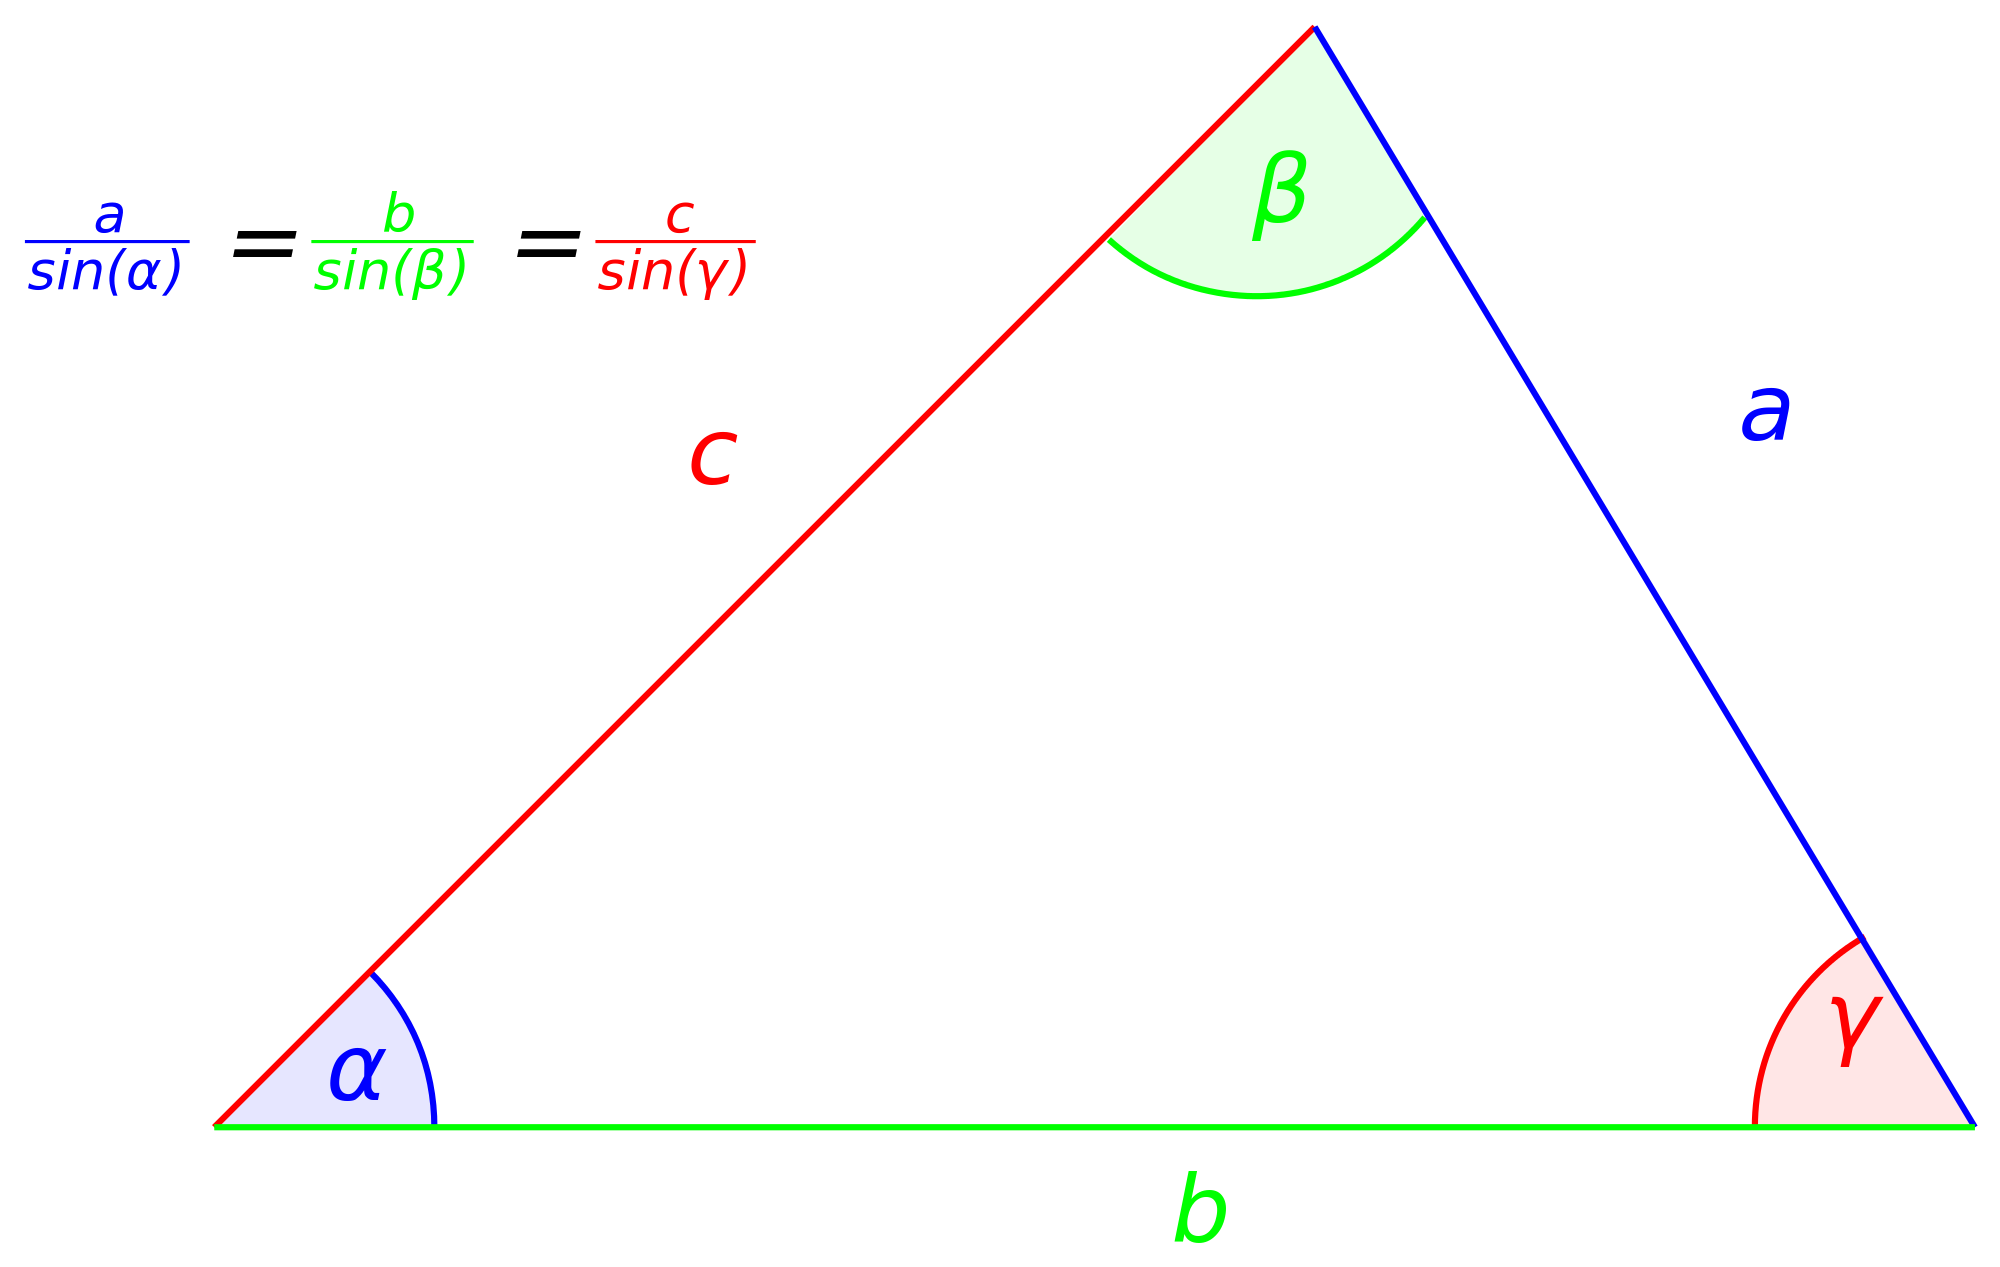
\includegraphics[width=0.5\textwidth]{images/sinussatz.png}
    \caption{Quelle: https://de.wikipedia.org/}
    
\end{figure}
\subsection{Cosinusssatz}
$a^2 + b^2 -2ab*cos(\gamma)= c^2$


\subsection{Standardintegrale}
\begin{minipage}{0.49\linewidth}
$\frac{d}{dx} arcsin(x) = \frac{1}{\sqrt{1-x^2}}$ \\
$\frac{d}{dx} arccos(x) = \frac{-1}{\sqrt{1-x^2}}$ \\
$\frac{d}{dx} arctan(x) =\frac {1}{x^2+1}$ \\
\end{minipage}
\begin{minipage}{0.49\linewidth}
$\frac{d}{dx} arsinh(x) =\frac{1}{\sqrt{x^2+1}}$ \\
$\frac{d}{dx} arcosh(x) =\frac{1}{\sqrt{x^2-1}}, $wenn $ x>1$ \\
$\frac{d}{dx} artanh(x) =\frac{1}{1-x^2}, $wenn $ |x|<1$ \\
\end{minipage}

\subsection{Euler Formel}
$exp(i \phi) = cos(\phi) + isin(\phi)$
\\
$exp(-i \phi) = cos(-\phi) + isin(-\phi) \Longleftrightarrow $ 
$exp(-i \phi) = cos(\phi) - isin(\phi)$ 

Daraus kann nun sin, sinh, cos und cosh in Termen von exp(x) ausgedrückt werden.

$\frac{exp(i \phi) + exp(-i \phi)}{2}  = cos(\phi)$\\
$\frac{exp(i \phi) - exp(-i \phi)}{2i}  = sin(\phi)$

Ignoriere alle i, dann folgt...

$\frac{exp(\phi) + exp(-\phi)}{2}  = cosh(\phi)$\\
$\frac{exp(\phi) - exp(-\phi)}{2}  = sinh(\phi)$




\subsection{Ableitungen, Integrale}
\subsection{Ableitungen}
$\frac{d}{dx}sin(x) = cos(x)$

$\frac{d}{dx}cos(x) = -sin(x)$

$\frac{d}{dx}tan(x) = \frac{d}{dx} \frac{sin(x)}{cos(x)} = \frac{cos(x)cos(x)- sin(x)sin(x)}{cos^2(x)} = 1 - \frac{sin^2(x)}{cos^2(x)} = 1 - tan^2(x) = \frac{1}{cos^2(x)}$

$\frac{d}{dx} \frac{1}{sin(x)} = \frac{0*sin(x) - 1*cos(x)}{sin^2(x)} = \frac{-cos(x)}{sin^2(x)}$ 

$\frac{d}{dx} \frac{1}{cos(x)} = \frac{0*cos(x) - 1*(-sin(x))}{cos^2(x)} = \frac{sin(x)}{cos^2(x)}$

$\frac{d}{dx}sin^2(x) = sin(x)*cos(x)+ cos(x)*sin(x) = 2*sin(x)*cos(x)$

$\frac{d}{dx}cos^2(x) = cos(x)*(-sin)(x)+ (-sin(x))*cos(x) = -2*sin(x)*cos(x)$ 
\newpage
\subsection{Rechenregeln}
\subsection{Additionstheoreme}
$sin^2(x)+cos^2(x) = 1$

$sin(x \pm y) = sin(x)cos(y) \pm cos(x)sin(y)$    \ \ $(\# umgekehrteAbleitungsregel)$

$cos(x \pm y) = cos(x)cos(y) \mp \sinx \siny$

$tan(x \pm y) = \frac{\tanx \pm \tany}{ 1 \mp \tanx \; \tany } = \frac{ sin(x \pm y) }{cos(x \pm y) }$

\subsection{Doppelwinkel}
$sin(2x)= 2\sinx \cosx = \frac{2 \tanx}{ 1 + tan^2(x) }$

$cos(2x)= cos^2(x) - sin^2(x) = 1 - 2sin^2(x) = 2cos^2(x) - 1 = \frac{ 1 - tan^2(x) }{ 1 + tan^2(x) }$

$tan(2x)= \frac{ 2 \tanx }{ 1 - tan^2(x) } = \frac{2}{ cot(x) - \tanx }$

$cot(2x)= \frac{ cot^2(x) - 1}{2cot(x)} = \frac{cot(x) - \tanx}{2}$ \\

Beweis mit Additionstheorem



\subsection{Produkt-zu-Summen-Formel}
$\sinx*sin(y) = \frac{1}{2}(cos(x-y)-cos(x+y))$

$\cosx*cos(y) = \frac{1}{2}(cos(x-y)+cos(x+y))$

$sin(x)*cos(y) = \frac{1}{2}(sin(x-y)+sin(x+y))$ \\



\subsection{Hyperbolische Funktionen}
$sinh(z) := \frac{e^z - e^{-z}}{2} = z + \frac{z^3}{3!} + \frac{z^5}{5!} + \frac{z^7}{7!} + \dots = \sum_{n=0}^\infty \frac{z^{2n+1}}{(2n+1)!}$

$cosh(z) := \frac{e^z + e^{-z}}{2}= 1 + \frac{z^2}{2!} + \frac{z^4}{4!} + \frac{z^6}{6!} + \dots = \sum_{n=0}^\infty \frac{z^{2n}}{(2n)!}$

$sin(z)= Im(e^{iz})=\dfrac{1}{2i} (e^{iz}-e^{-iz})$ \\

$cos(z)=\text{Re}(e^{iz})=\dfrac{1}{2}(e^{iz}+e^{-iz})$ \\

$sinh(\pm iz) = \pm i \cdot \sin(z)$\\
$cosh(\pm iz) = cos(z)$\\
$sin(iz)= i\cdot sinh(z)$\\
$cos(iz)=cosh(z)$\\

$ \sin(-z) = - \sin(z) $\\
$ \tan-(z) = -\tan(z) $\\
$ \cos(-z) = \cos(z) $ \\
$ \arctan(-z) = -\arctan(z) $

$\sin(z) = \sin(x)\cosh(y) + i\cos(x)\sinh(y)$\\
$\cos(z) = \cos(x)\cosh(y) - i\sin(x)\sinh(y)$\\
$e^z = e^x \cos(y) + i e^x \sin(y)$\\
$\sinh(z) = \cos(y)\sinh(x) + i\sin(y)\cosh(x)$\\
$\cosh(z) = \cos(y)\cosh(x) + i\sin(y)\sinh(x)$	

\begin{itemize}[leftmargin=*]
	\item $\int \sinh(ax + b) \,dx = \frac{\cosh(ax + b)}{a}$; $\int \sinh(x) \,dx
	= \cosh(x)$
	\item $\int \cosh(ax + b) \,dx = \frac{\sinh(ax + b)}{a}$; $\int \cosh(x) \,dx
	= \sinh(x)$
	\item $\int \tan(ax + b) \,dx = \frac{\log(\cosh(ax+b))}{a}$; $\int \tan(x)
	\,dx = \log(\cosh(x))$
\end{itemize}


\subsection{Additionstheoreme}
$sinh(z_1 \pm z_2) = sinh(z_1) \cdot cosh(z_2) \pm sinh(z_2) \cdot cosh(z_1)$

$cosh(z_1 \pm z_2) = cosh(z_1) \cdot cosh(z_2) \pm sinh(z_1) \cdot sinh(z_2)$

$tanh(z_1 \pm z_2) = \frac{tanh(z_1) \pm tanh(z_2)}{1 \pm tanh(z_1) \cdot tanh(z_2)}$


\subsubsection{Zusammenhänge}
$cosh^2(z) - sinh^2(z) = 1$ \hfill $cosh(z) + sinh(z) = e^z$ \hfill $cosh(z) - sinh(z) = e^{-z}$

\subsection{Ableitungen}
$\frac{d}{dz}sinh(z) = cosh(z)$ \hfill $\frac{d}{dz}cosh(z) = sinh(z)$ \hfill $\frac{d}{dz}tanh(z) = 1 -tanh^2(z) = \frac{1}{cosh^2(x)}$

\section{Plots Trigonometrischer Funktionen}
%Alle Plots in diesem Kapitel von www.wikipedia.org!

\begin{figure}[!htb]
	\centering
	\begin{minipage}{.5\textwidth}
		\centering
		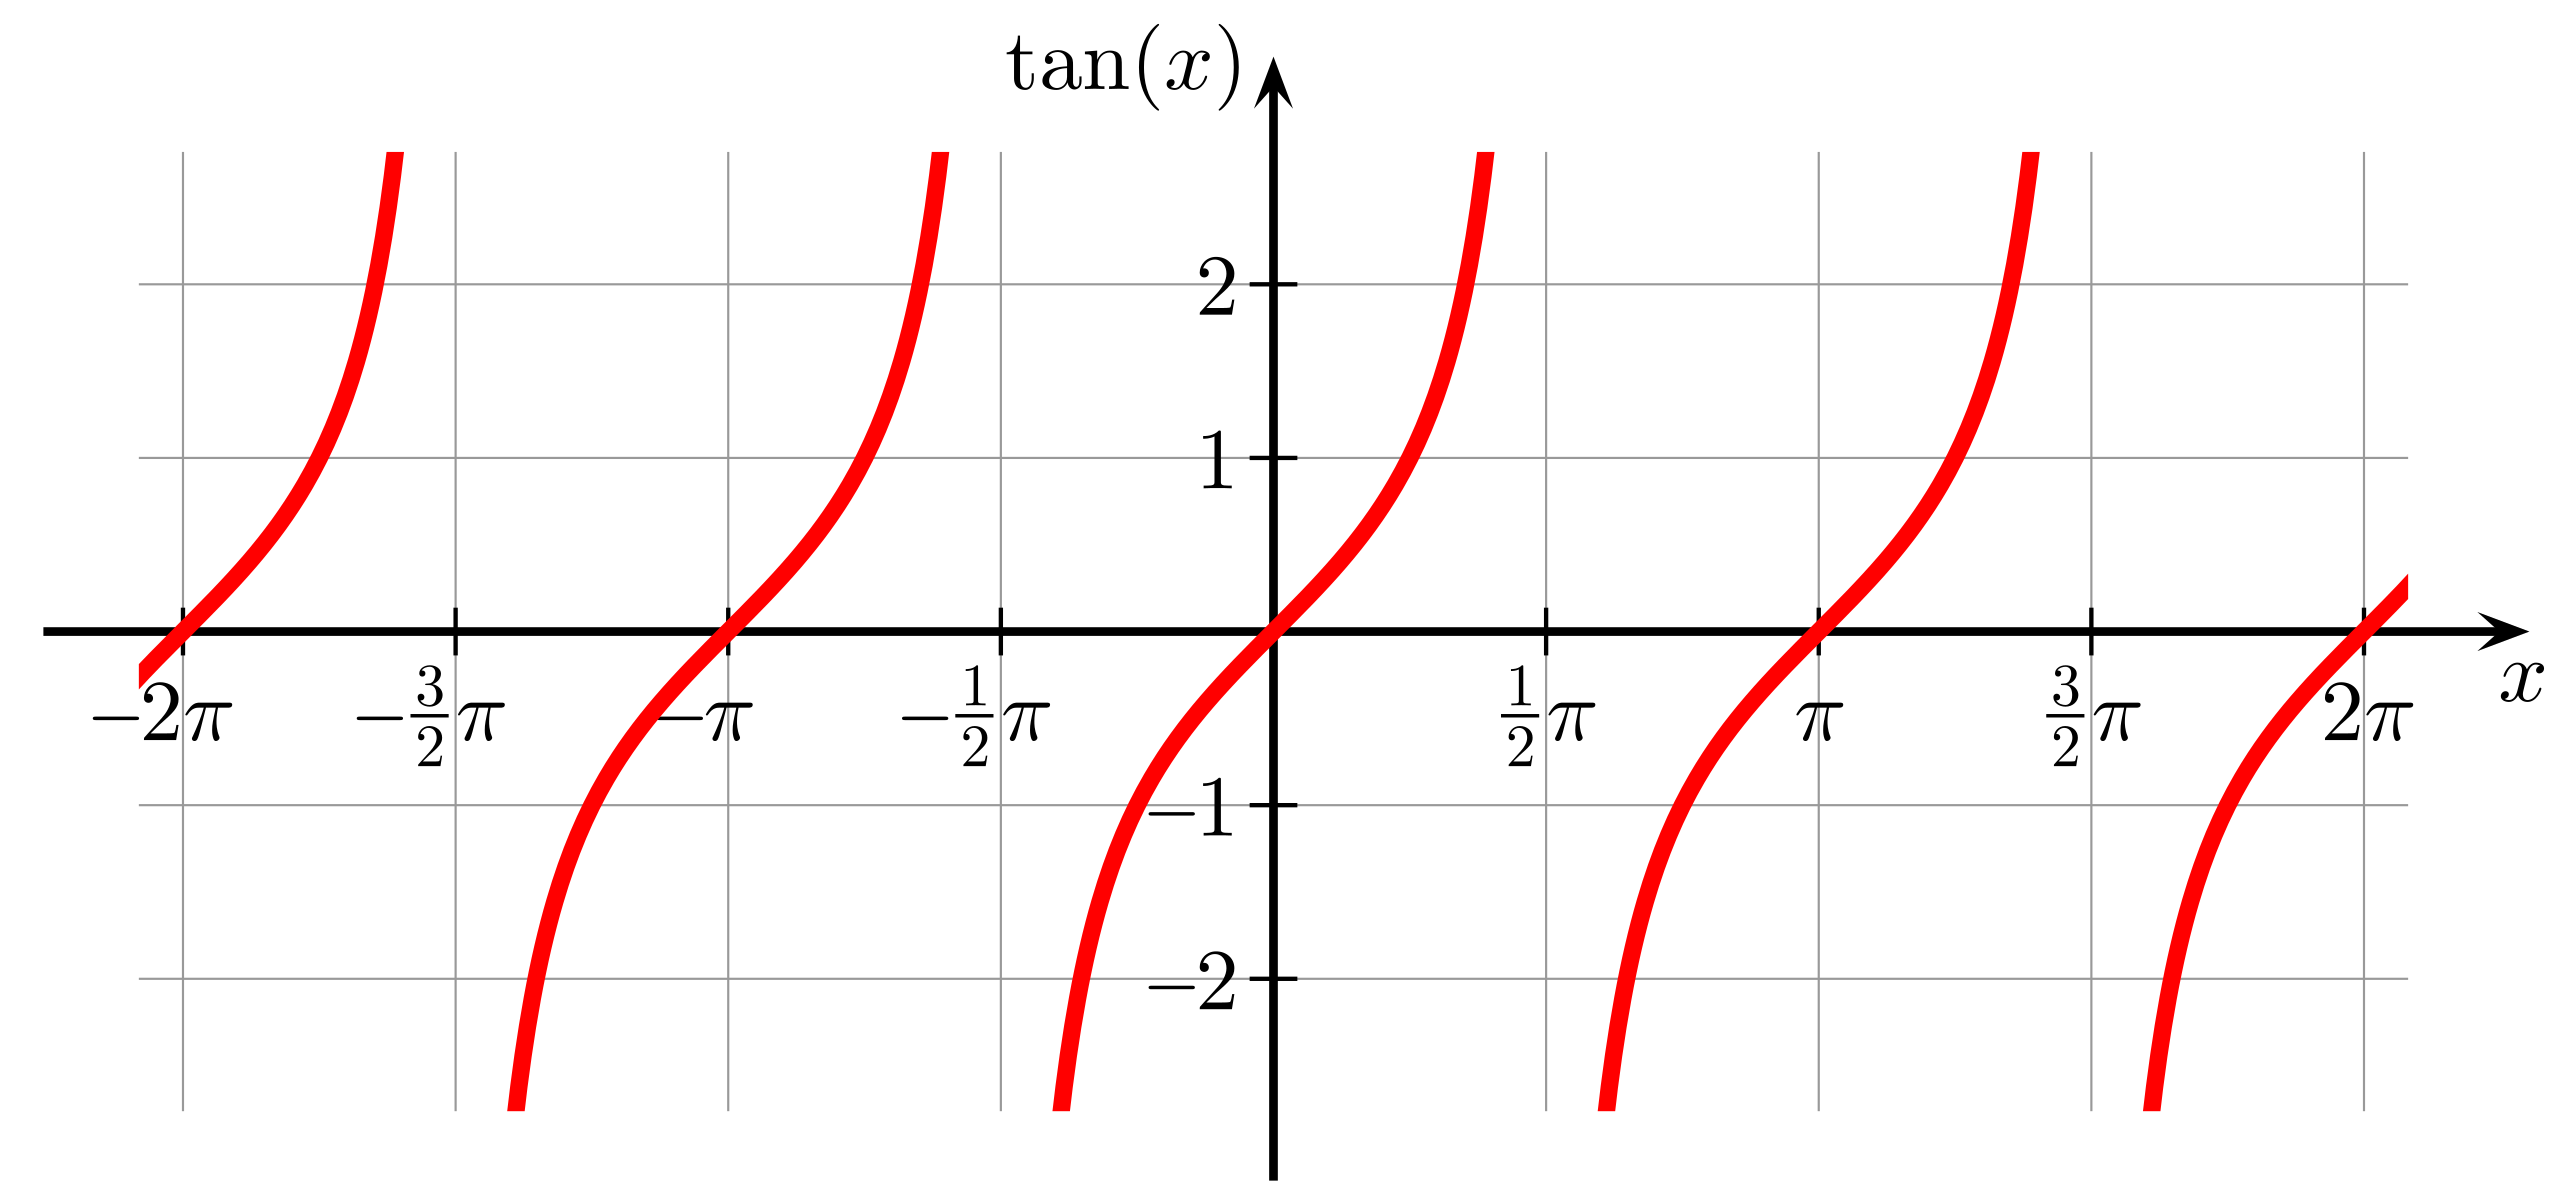
\includegraphics[width=1\linewidth]{images/tan.png}
	\end{minipage}%
	\begin{minipage}{0.5\textwidth}
		\centering
		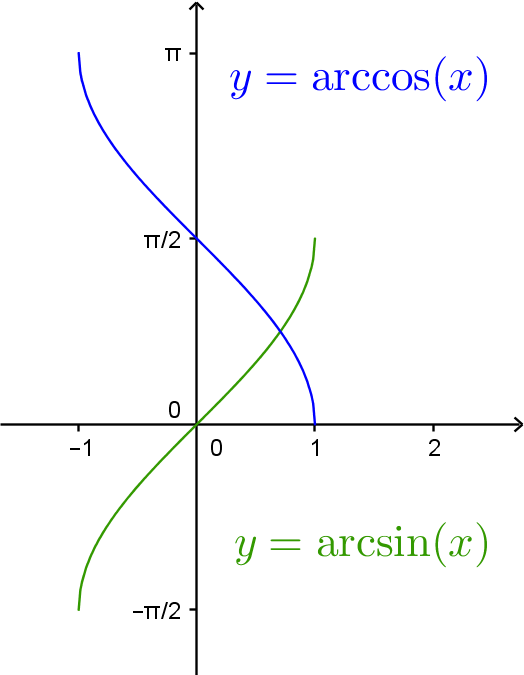
\includegraphics{images/asinacos.png}
	\end{minipage}
\end{figure}


\begin{figure}[H] 
	\centering
	{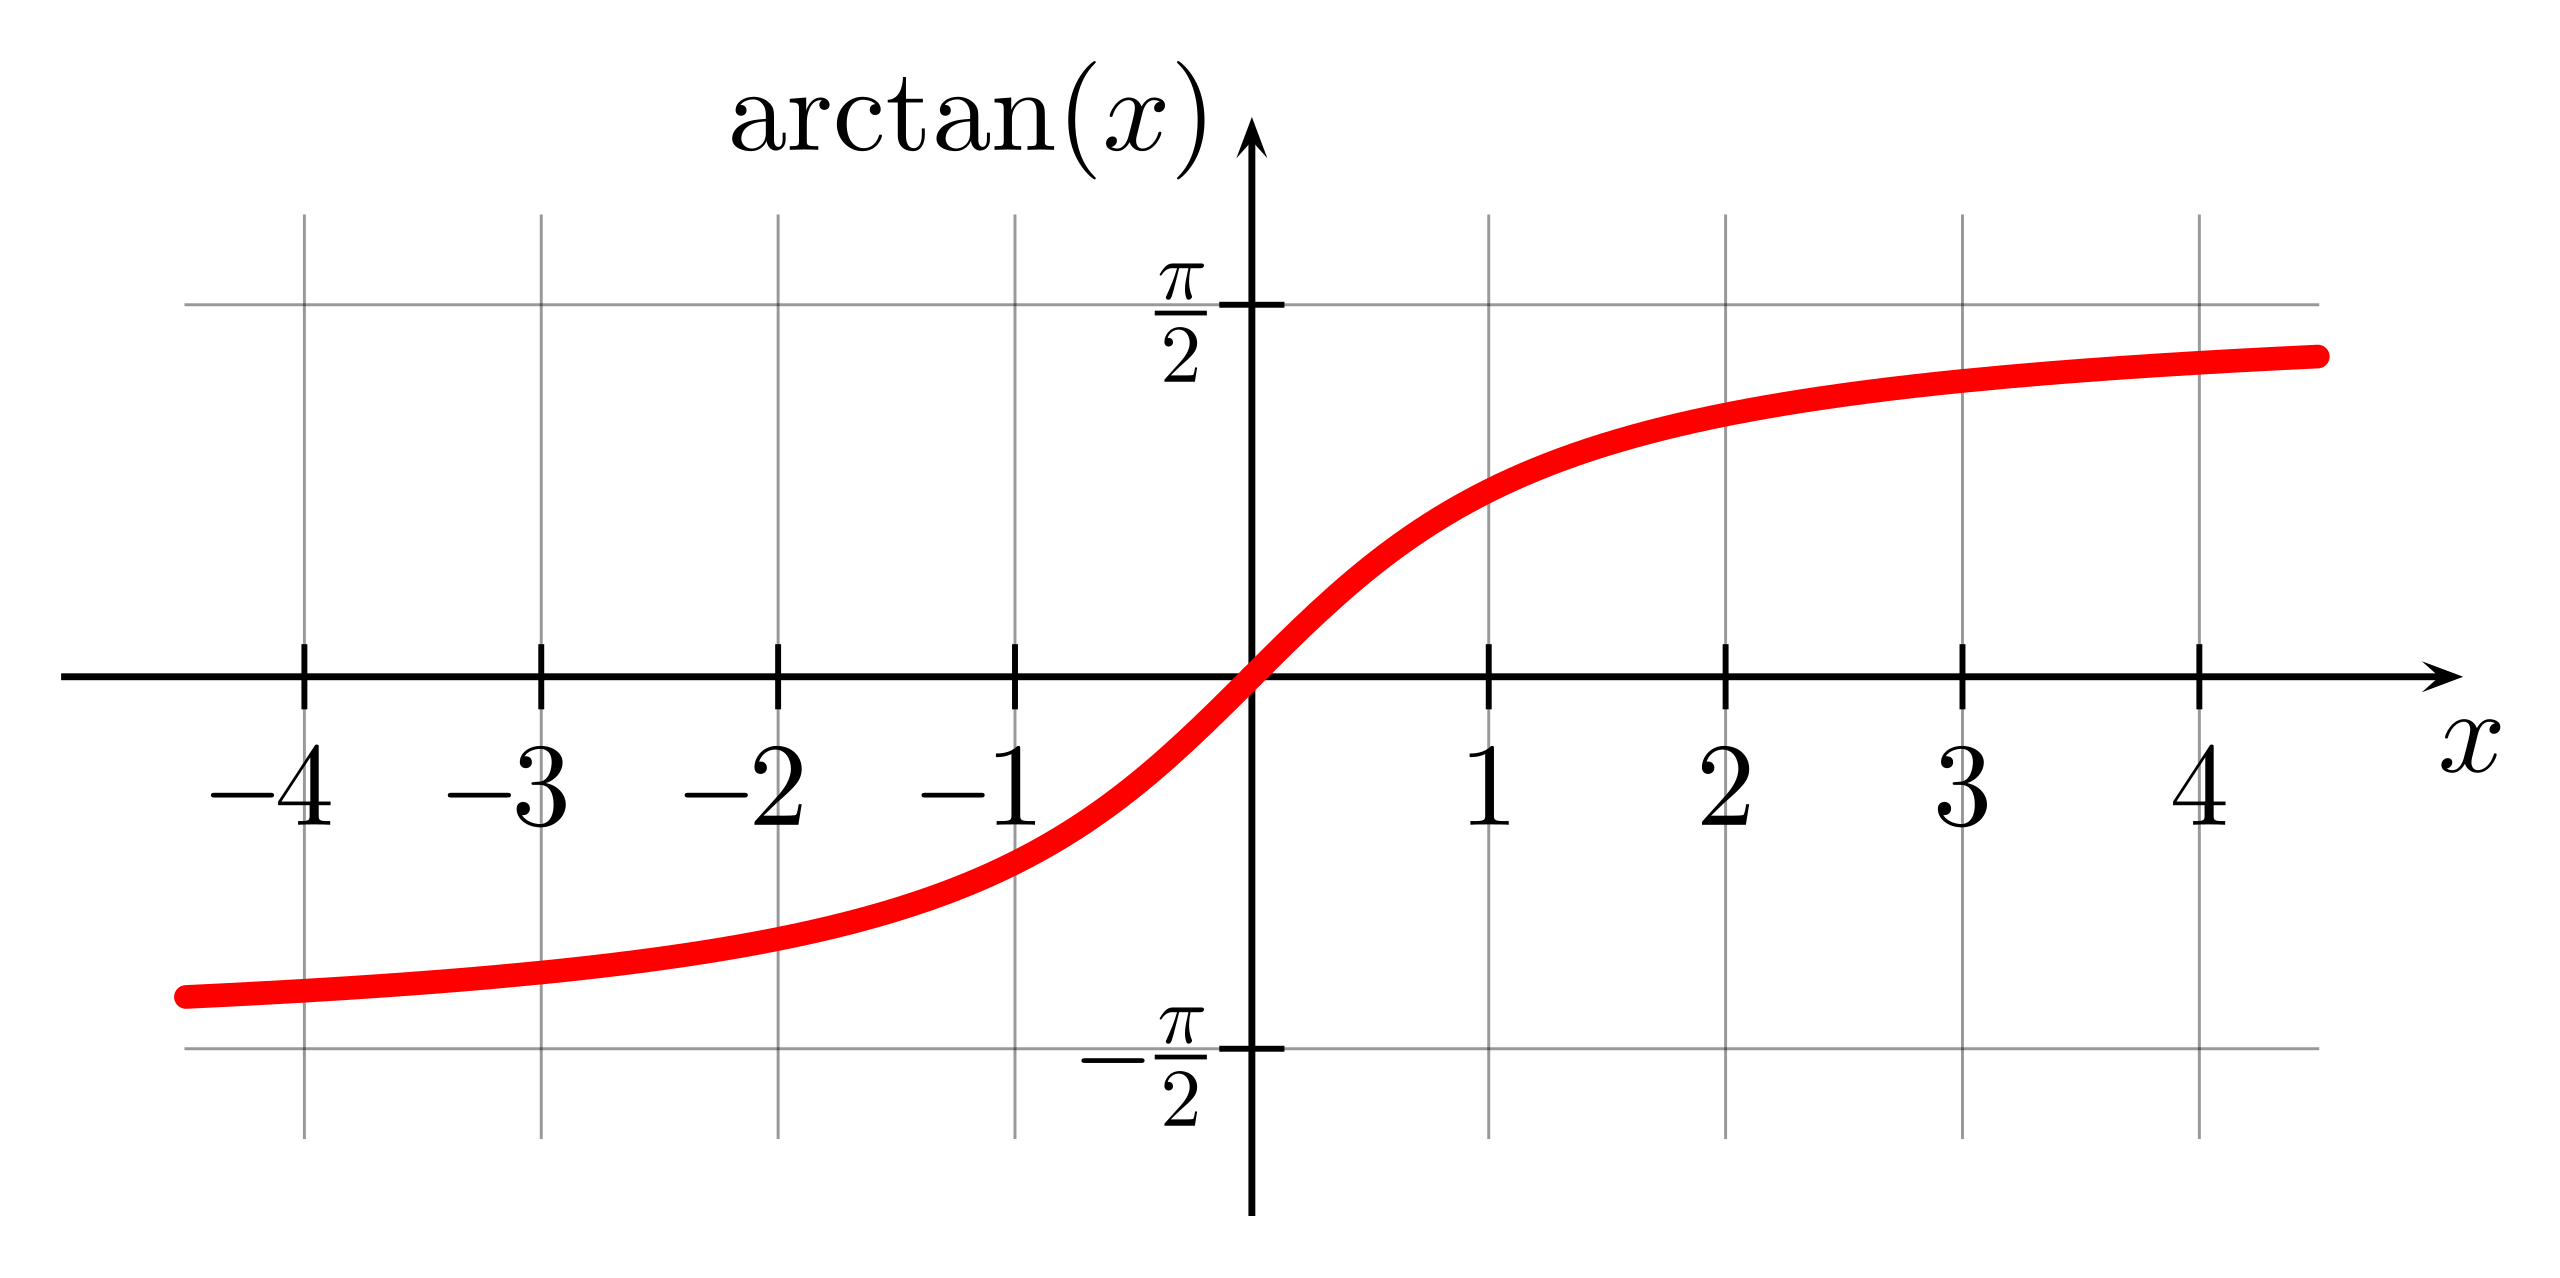
\includegraphics[width=0.55\textwidth]{images/arctan.png}}
\end{figure}



\begin{figure}[!htb]
	\centering
	\begin{minipage}{.5\textwidth}
		\centering
		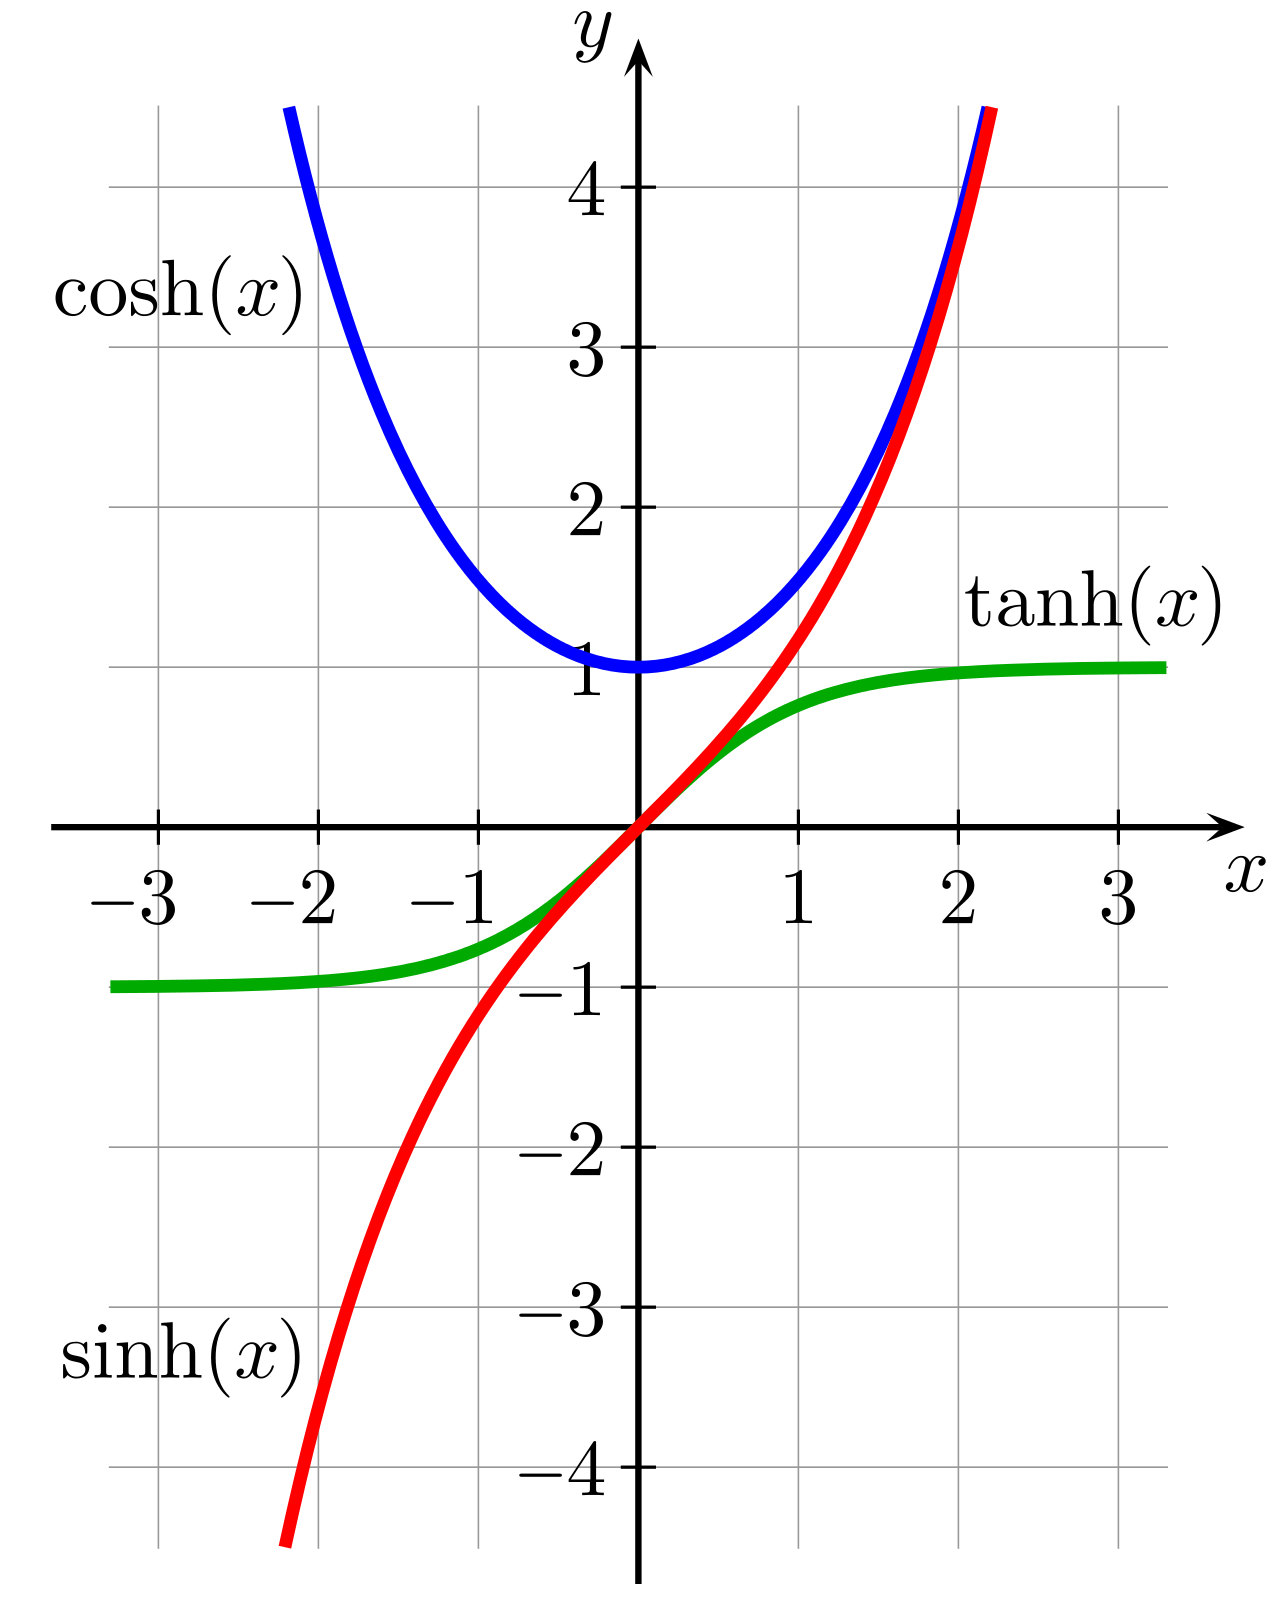
\includegraphics[width=1\linewidth]{images/sinhcoshtanh.png}
	\end{minipage}%
	\begin{minipage}{.5\textwidth}
		\centering
		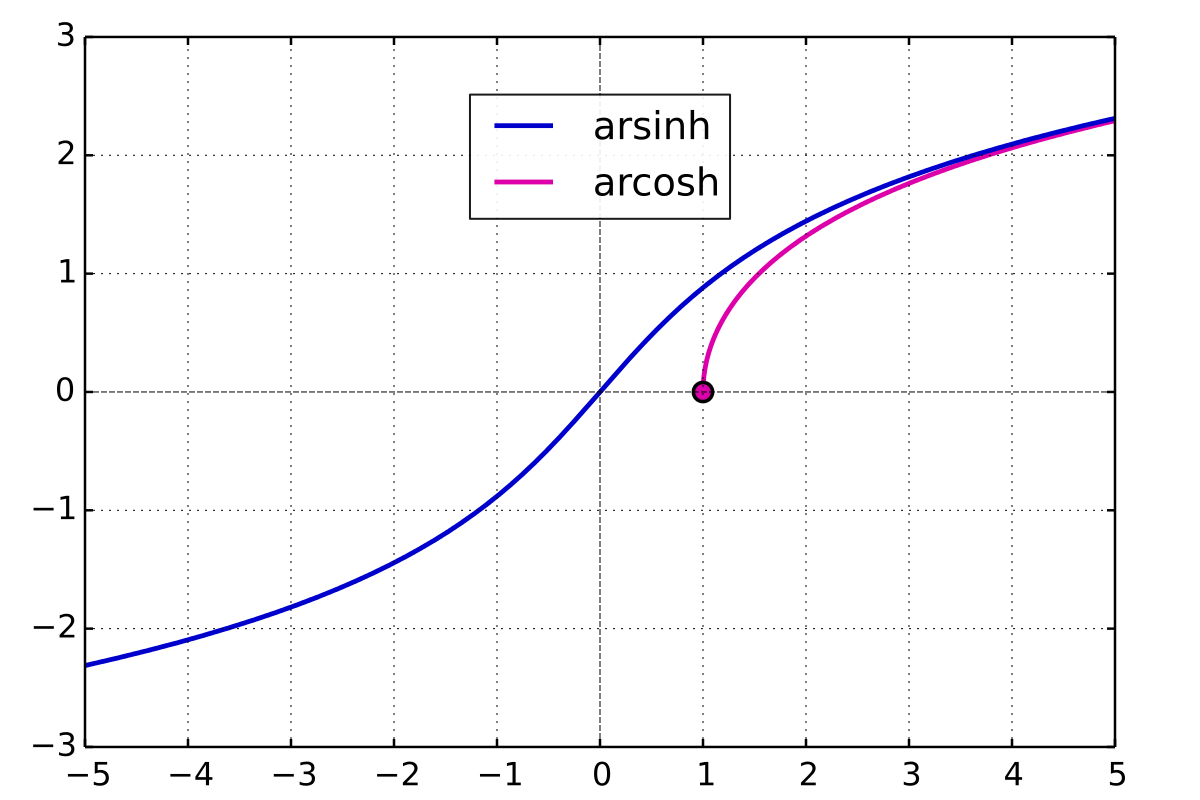
\includegraphics[width=1\linewidth]{images/arsinharcosh.png}
	\end{minipage}
\end{figure}

